\documentclass[tikz,border=10pt]{standalone}
\usepackage{tikz}
\usetikzlibrary{shapes, arrows, positioning, calc}

\begin{document}

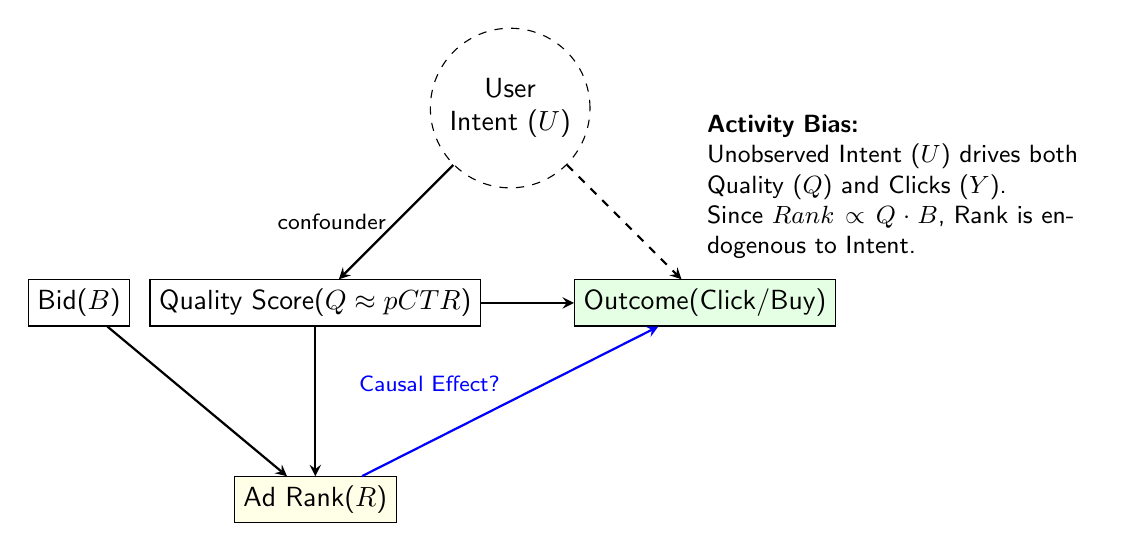
\begin{tikzpicture}[node distance=2.5cm, auto, >=stealth]
    % Nodes
    \node (intent) [circle, draw, dashed, align=center, font=\sffamily] {User\\Intent ($U$)};
    \node (quality) [rectangle, draw, below left of=intent, node distance=3.5cm, font=\sffamily] {Quality Score\\($Q \approx pCTR$)};
    \node (bid) [rectangle, draw, left of=quality, node distance=3cm, font=\sffamily] {Bid\\($B$)};
    \node (rank) [rectangle, draw, below of=quality, fill=yellow!10, font=\sffamily] {Ad Rank\\($R$)};
    \node (click) [rectangle, draw, below right of=intent, node distance=3.5cm, fill=green!10, font=\sffamily] {Outcome\\(Click/Buy)};

    % Edges
    \draw[->, thick] (intent) -- node[left, font=\footnotesize\sffamily] {confounder} (quality);
    \draw[->, thick, dashed] (intent) -- (click);
    \draw[->, thick] (bid) -- (rank);
    \draw[->, thick] (quality) -- (rank);
    \draw[->, thick, blue] (rank) -- node[midway, fill=white, font=\footnotesize\sffamily] {Causal Effect?} (click);
    \draw[->, thick] (quality) -- (click); % True relevance affects click obviously

    % Labels
    \node[right of=intent, text width=5cm, font=\small\sffamily, xshift=2.5cm, yshift=-1cm] {
        \textbf{Activity Bias:}\\
        Unobserved Intent ($U$) drives both Quality ($Q$) and Clicks ($Y$).\\
        Since $Rank \propto Q \cdot B$, Rank is endogenous to Intent.
    };
\end{tikzpicture}

\end{document}
